\documentclass{article}
\usepackage[utf8]{inputenc}
\usepackage{amsmath}
\usepackage{graphicx}
\usepackage{geometry} % <-- FIX 1: Added the missing geometry package
\usepackage{hyperref}
\usepackage{listings}
\usepackage{float}
\usepackage{booktabs} % For professional looking tables

\geometry{a4paper, margin=1in}

\title{Hardware Project: PT-100 Temperature Sensor Analysis}
\author{Divyansh (EE25BTECH11037) \and Shriyansh (EE25BTECH11052)}
\date{\today}

\begin{document}
	
	\maketitle
	
	\begin{abstract}
		This report details a project aimed at measuring and analyzing the voltage output of a PT-100 platinum resistance temperature detector (RTD) at varying temperatures. The project involves setting up a circuit with an Arduino, collecting data, and fitting it to a theoretical model using the least squares method. The experiment successfully demonstrates the functionality of the PT-100 sensor for precise temperature measurement and verifies its linear relationship between temperature and resistance (and consequently voltage).
	\end{abstract}
	
	\section{Aim}
	To measure and analyze the voltage output of a PT-100 sensor at varying temperatures.
	
	\section{Components Required}
	\begin{enumerate}
		\item Breadboard
		\item Arduino UNO
		\item PT-100 Sensor
		\item Resistor (300 $\Omega$)
		\item Jumper Cables
		\item Electric Kettle
		\item Thermometer
	\end{enumerate}
	
	\section{Introduction to PT-100 Sensor}
	A PT-100 is a platinum resistance temperature detector (RTD). The resistance of the platinum element changes with temperature. The "PT" stands for platinum, and "100" indicates that it has a resistance of 100 $\Omega$ at 0°C.
	
	\section{Procedure}
	
	\subsection{Connections}
	The circuit components were arranged as shown in the diagram below. The PT-100 sensor and a 300 $\Omega$ resistor were set up in a voltage divider configuration, with the Arduino's analog input pin (A0) used to measure the voltage across the PT-100.
	
\begin{figure}[H]
	\centering
	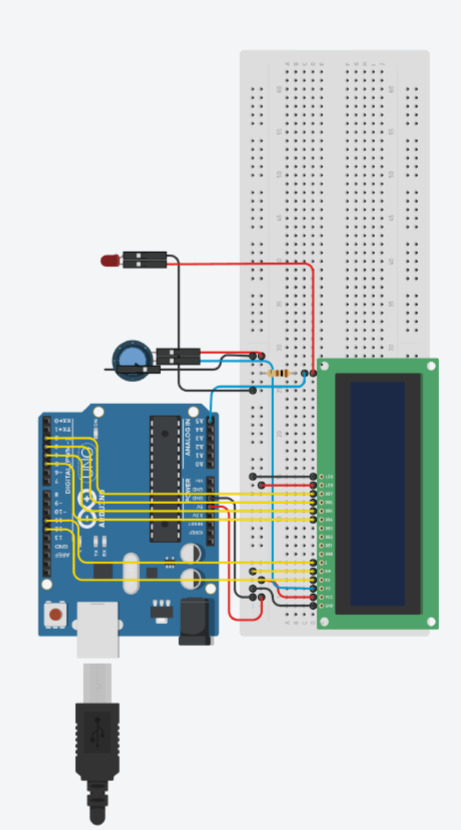
\includegraphics[width=0.8\textwidth]{../figs/circuit}
	\caption{Circuit Diagram and Breadboard Setup.}
	\label{fig:circuit}
\end{figure}
	
	An electric kettle was used to heat water, thereby increasing the temperature of the PT-100 sensor immersed in it. The corresponding voltage values were measured using the Arduino setup.
	
	\subsection{Code}
	The following C++ code was uploaded to the Arduino UNO to read the sensor values.
	
	\begin{lstlisting}[language=C++, caption={Arduino Code for Reading Sensor Voltage}, label={lst:code}]
		#include "Arduino.h"
		
		void setup() {
			Serial.begin(9600);
		}
		
		void loop() {
			int sensorValue = analogRead(A0);
			double voltage = (5.0 * sensorValue) / 1023.0;
			Serial.println(voltage);
			delay(1000);
		}
	\end{lstlisting}
	
	\subsubsection*{Code Explanation}
	\begin{itemize}
		\item \textbf{setup():} The \texttt{Serial.begin(9600)} function initializes serial communication at a baud rate of 9600 bits per second (bps). This allows the Arduino to send data to the serial monitor.
		\item \textbf{loop():} This function runs continuously.
		\begin{itemize}
			\item \texttt{analogRead(A0)} reads the voltage from the analog pin A0, where the sensor is connected. The analog-to-digital converter (ADC) returns a value between 0 and 1023.
			\item This raw sensor value is converted to an approximate voltage using the formula:
			\[
			\text{Voltage} = \frac{5.0 \times \text{sensorValue}}{1023.0}
			\]
			This maps the ADC's 0-1023 range to the Arduino's 0-5V range.
			\item \texttt{Serial.println(voltage)} sends the calculated voltage to the serial monitor.
			\item \texttt{delay(1000)} pauses the loop for 1000 milliseconds (1 second) before the next reading.
		\end{itemize}
	\end{itemize}
	
	\section{Theory}
	The relationship between temperature and the resistance of a platinum sensor can be described by the Callendar-Van Dusen equation. For this project, we model the output voltage \(V(T)\) as a function of temperature \(T\) (in °C) using a simplified polynomial form:
	\[
	V(T) = V_0 \left(1 + AT + BT^2\right)
	\]
	This can be rewritten in a linear matrix form suitable for the least squares method.
	\[
	C = n^T x
	\]
	where:
	\[ C = V(T), \quad x = \begin{pmatrix} 1 \\ T \\ T^2 \end{pmatrix}, \quad n = \begin{pmatrix} V(0) \\ A \cdot V(0) \\ B \cdot V(0) \end{pmatrix} \]
	
	For multiple data points \((T_i, V(T_i))\), the system of equations is given by:
	\[ Xn = c \]
	where:
	\[ X = \begin{pmatrix} 1 & T_1 & T_1^2 \\ 1 & T_2 & T_2^2 \\ \vdots & \vdots & \vdots \\ 1 & T_n & T_n^2 \end{pmatrix}, \quad c = \begin{pmatrix} V(T_1) \\ V(T_2) \\ \vdots \\ V(T_n) \end{pmatrix} \]
	
	\subsection{The Theory of Least Squares}
	The matrix equation \(Xn = c\) is an overdetermined system because the number of data points is typically greater than the number of unknown coefficients. An exact solution does not exist. The goal of the least squares method is to find the vector \(n\) that minimizes the sum of the squared errors between the model's prediction and the actual measured voltages.
	
	The error vector \(e\) is defined as:
	\[ e = c - Xn \]
	We want to minimize the squared Euclidean norm of this error, \( \|e\|^2 \). This leads to the normal equations:
	\[ X^T X n = X^T c \]
	Assuming that \(X^T X\) is invertible, we can solve for \(n\):
	\[ n = (X^T X)^{-1} X^T c \]
	This is the fundamental equation of the least squares method, which provides the best-fit coefficients.
	
	From our experimental data and applying the least squares method, we get the coefficient vector \(n\):
	\[ n = \begin{pmatrix} 1.2482 \\ 4.1397 \times 10^{-3} \\ -7.0833 \times 10^{-6} \end{pmatrix} \]
	
	\section{Results}
	
	\subsection{Training Data}
	\begin{table}[H]
		\centering
		\caption{Training Data: Measured Voltage at Different Temperatures.}
		\label{tab:trainingdata}
		% This is a LaTeX table.
\documentclass{article}
% You can include this in your main .tex document using % This is a LaTeX table.
\documentclass{article}
% You can include this in your main .tex document using % This is a LaTeX table.
\documentclass{article}
% You can include this in your main .tex document using \input{training_data.tex}
% Or copy the \begin{table}...\end{table} block into your document.

\begin{document}
% This is a LaTeX table with full grid lines.
% You'll need the \usepackage{array} package in your preamble for the formatting.

% This is a LaTeX table with full grid lines.
% You'll need the \usepackage{array} package in your preamble for the formatting.

\begin{table}[h]
\centering
\caption{Training Data}
\label{tab:training_data}
\begin{tabular}{|c|c|}
\hline
\textbf{Temperature ($^{\circ}$C)} & \textbf{Voltage (V)} \\
\hline
25.1 & 2.15543 \\
\hline
25.9 & 2.16031 \\
\hline
34.5 & 2.19941 \\
\hline
36.1 & 2.20430 \\
\hline
40.0 & 2.21408 \\
\hline
46.3 & 2.24340 \\
\hline
51.1 & 2.26295 \\
\hline
53.1 & 2.26784 \\
\hline
59.1 & 2.29228 \\
\hline
62.9 & 2.30694 \\
\hline
68.2 & 2.32649 \\
\hline
74.8 & 2.35093 \\
\hline
80.4 & 2.37048 \\
\hline
89.0 & 2.39980 \\
\hline
90.3 & 2.40469 \\
\hline
92.0 & 2.40958 \\
\hline
95.8 & 2.42424 \\
\hline
97.3 & 2.42913 \\
\hline
\end{tabular}
\end{table}
\end{document}
% Or copy the \begin{table}...\end{table} block into your document.

\begin{document}
% This is a LaTeX table with full grid lines.
% You'll need the \usepackage{array} package in your preamble for the formatting.

% This is a LaTeX table with full grid lines.
% You'll need the \usepackage{array} package in your preamble for the formatting.

\begin{table}[h]
\centering
\caption{Training Data}
\label{tab:training_data}
\begin{tabular}{|c|c|}
\hline
\textbf{Temperature ($^{\circ}$C)} & \textbf{Voltage (V)} \\
\hline
25.1 & 2.15543 \\
\hline
25.9 & 2.16031 \\
\hline
34.5 & 2.19941 \\
\hline
36.1 & 2.20430 \\
\hline
40.0 & 2.21408 \\
\hline
46.3 & 2.24340 \\
\hline
51.1 & 2.26295 \\
\hline
53.1 & 2.26784 \\
\hline
59.1 & 2.29228 \\
\hline
62.9 & 2.30694 \\
\hline
68.2 & 2.32649 \\
\hline
74.8 & 2.35093 \\
\hline
80.4 & 2.37048 \\
\hline
89.0 & 2.39980 \\
\hline
90.3 & 2.40469 \\
\hline
92.0 & 2.40958 \\
\hline
95.8 & 2.42424 \\
\hline
97.3 & 2.42913 \\
\hline
\end{tabular}
\end{table}
\end{document}
% Or copy the \begin{table}...\end{table} block into your document.

\begin{document}
% This is a LaTeX table with full grid lines.
% You'll need the \usepackage{array} package in your preamble for the formatting.

% This is a LaTeX table with full grid lines.
% You'll need the \usepackage{array} package in your preamble for the formatting.

\begin{table}[h]
\centering
\caption{Training Data}
\label{tab:training_data}
\begin{tabular}{|c|c|}
\hline
\textbf{Temperature ($^{\circ}$C)} & \textbf{Voltage (V)} \\
\hline
25.1 & 2.15543 \\
\hline
25.9 & 2.16031 \\
\hline
34.5 & 2.19941 \\
\hline
36.1 & 2.20430 \\
\hline
40.0 & 2.21408 \\
\hline
46.3 & 2.24340 \\
\hline
51.1 & 2.26295 \\
\hline
53.1 & 2.26784 \\
\hline
59.1 & 2.29228 \\
\hline
62.9 & 2.30694 \\
\hline
68.2 & 2.32649 \\
\hline
74.8 & 2.35093 \\
\hline
80.4 & 2.37048 \\
\hline
89.0 & 2.39980 \\
\hline
90.3 & 2.40469 \\
\hline
92.0 & 2.40958 \\
\hline
95.8 & 2.42424 \\
\hline
97.3 & 2.42913 \\
\hline
\end{tabular}
\end{table}
\end{document} % <-- FIX 3: Simplified the file path
	\end{table}
	
\begin{figure}[H]
	\centering
	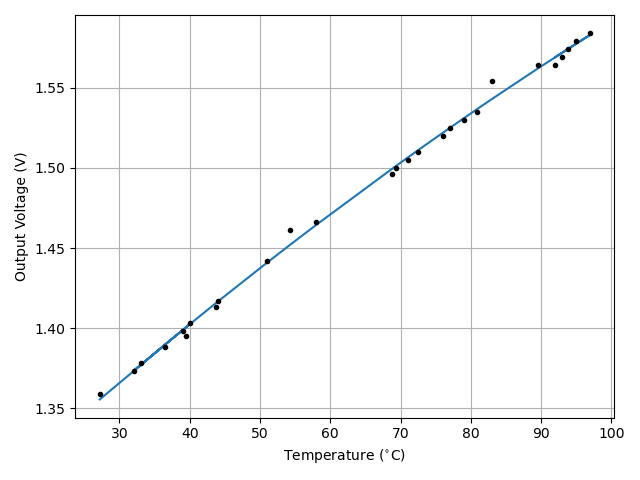
\includegraphics[width=1\textwidth]{../figs/train}
	\caption{Output Voltage vs. Temperature for Training Data.}
	\label{fig:train}
\end{figure}

\begin{table}[H]
	\centering
	\caption{Validation Data.} % <-- Corrected caption
	\label{tab:validationdata} % <-- FIX 2: Fixed the duplicate label
	\begin{tabular}{cc}
	\toprule
	\textbf{Temp (°C)} & \textbf{Voltage (V)} \\
	\midrule
	27.2 & 1.359 \\
	36.5 & 1.388 \\
	39.5 & 1.395 \\
	51.0 & 1.442 \\
	68.8 & 1.496 \\
	72.5 & 1.510 \\
	79.0 & 1.530 \\
	89.6 & 1.564 \\
	93.8 & 1.574 \\
	\bottomrule
\end{tabular} % <-- FIX 3: Pointed to the correct file and simplified path
\end{table}


\begin{figure}[H]
	\centering
	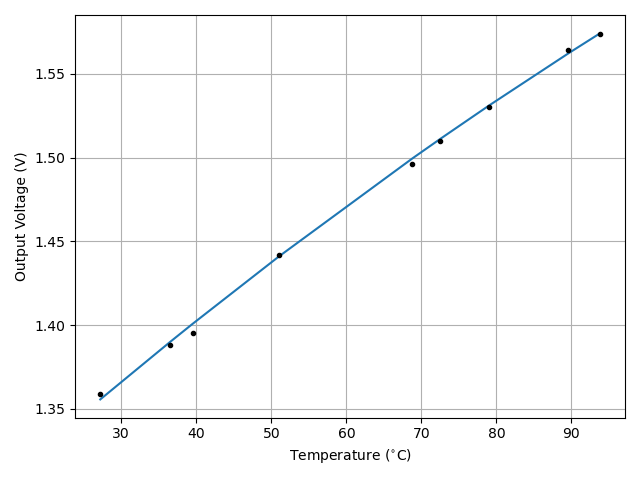
\includegraphics[width=1\linewidth]{../figs/valid}
	\caption{Validation Data}
	\label{fig:valid}
\end{figure}

	
	\section{Model Concavity and Optimization Choice}
	An important observation is that the coefficient of the \(T^2\) term (\(B \cdot V(0)\)) is negative ($-7.0833 \times 10^{-6}$). This means the governing function \(V(T)\) is strictly concave. This has a significant implication from a machine learning perspective.
	
	Many optimization problems in machine learning are solved using gradient descent, an iterative algorithm that finds the minimum of a function. Gradient descent works by taking steps in the direction of the negative gradient of the function. This process is guaranteed to find the global minimum only if the function is convex.
	
	Since our function is concave, it has a maximum, not a minimum. Applying gradient descent here would fail to find the correct parameters because the algorithm is designed to minimize a cost function, not maximize it. Therefore, the analytical least squares method, which directly solves for the optimal parameters via the normal equations, is the appropriate and more robust choice for this linear regression problem.
	
	\section{Conclusion}
	In conclusion, this report successfully demonstrates the use of the PT-100 sensor with an Arduino for temperature measurement. The project involved setting up a circuit, coding, and data collection to observe the sensor's response across varying temperatures. The experiment verified the PT-100's effectiveness in providing reliable temperature readings, making it a valuable component for precise temperature monitoring in various applications.
	
\end{document}